\documentclass[]{article}

\usepackage{mathtools,mathrsfs,url,fancyhdr, graphicx,amssymb}

\renewcommand{\headrulewidth}{0pt}
\fancyhead[L]{}
\fancyhead[C]{
	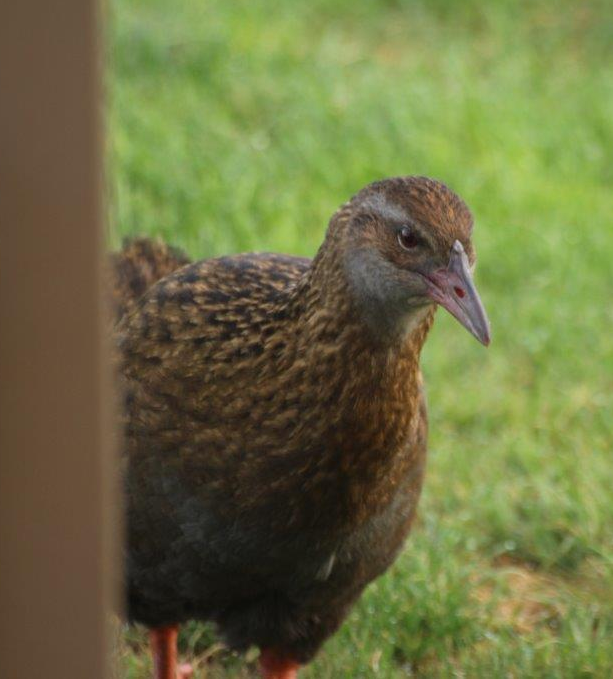
\includegraphics[width=2cm]{weka.png}
}


\graphicspath{ {images/} }
\newcommand{\Lagr}{\mathscr{L}}
\pagestyle{plain}

%opening
\title{Introduction into General Relativity\\Assignment 3--Problem 1\\The stress--energy tensor $T^{\mu\nu}$ for the dust}
\author{Simon Crase}

\begin{document}

\maketitle
\thispagestyle{fancy}
\begin{abstract}
I haven't made a lot of headway this week, but I've decided to submit what little I have and move on, as the lectures in the next few weeks are what I'm really looking for.


\end{abstract}

\section{Variation of the Action}

For the dust, \cite{akhmedev2016} gives the following.
\begin{align}
S_M &= - \sum_{q=1}^N m_q \, \int d\tau \, \sqrt{g_{\mu\nu}[z_q(\tau)] \, \dot{z}_q^\mu(\tau)\, \dot{z}_q^\nu(\tau)}\\
&=- \sum_{q=1}^N \int d^{4}(x) \sqrt{|g(x)|} \int d\tau\frac{\delta^{(4)}(x-z(\tau))}{ \sqrt{|g(z)|}} m_{q} \sqrt{ g_{\mu\nu}(z) \dot{z}_{q}^{\mu} \dot{z}_{q}^{\nu}}\\
&= \int d^{4}(x) \sqrt{|g(x)|} \int d\tau\frac{\delta^{(4)}(x-z(\tau))}{ \sqrt{|g(z)|}} \Big\{ - \sum_{q=1}^N m_{q} \sqrt{ g_{\mu\nu}(z) \dot{z}_{q}^{\mu} \dot{z}_{q}^{\nu}}\Big\}\\
&= \int d^{4}(x) \sqrt{|g(x)|} \Lagr  \text{   where $\Lagr$ is defined by (\ref{eq:L})}
\end{align}

\begin{align}
\Lagr &\triangleq \int d\tau\frac{\delta^{(4)}(x-z(\tau))}{ \sqrt{|g(z)|}} \Big\{ - \sum_{q=1}^N m_{q} \sqrt{ g_{\mu\nu}(z) \dot{z}_{q}^{\mu} \dot{z}_{q}^{\nu}}\Big\} \label{eq:L}\\
&= -\sum_{q=1}^N \sqrt{g_{\mu\nu}(z)\frac{m_q}{ \sqrt{|g(z)|}} \dot{z}_{q}^{\mu} \frac{m_q}{ \sqrt{|g(z)|}} \dot{z}_{q}^{\nu}}  \label{eq:L2}
\end{align}
(\ref{eq:L2}) follows from the integral form of the Dirac delta function given in \cite{wiki_delta}.  $\Lagr$ can be expressed more concisely by using the momentum $p^{\nu}\triangleq\frac{m_q}{ \sqrt{|g(z)|}} \dot{z}_{q}^{\nu}$
\begin{align}
\Lagr &= -\sum_{q=1}^N \sqrt{g_{\mu\nu}(z) p^{\mu}_q p^{\nu}_q} \\
&= -\sum_{q=1}^N \sqrt{g^{\mu\nu}(z) p_{q,\mu} p_{q,\nu}} \\
&= -\sum_{q=1}^N \sqrt{ p^{\mu}_q p_{q,\mu}}
\end{align}
Hence
\begin{align}
\delta_{g}S_m &= \delta_{g}  \int d^{4}(x) \sqrt{|g(x)|} \Lagr\\
&= \int d^{4}(x) \sqrt{|g(x)|} \Big[ \frac{\partial \Lagr}{\partial g^{\mu\nu}}-\frac{1}{2}\Lagr g_{\mu\nu}\Big] \delta_{g^{\mu\nu}}\\
&= \int d^{4}(x) \sqrt{|g(x)|} T_{\mu\nu} \delta_{g^{\mu\nu}} 
\end{align}
Where $T_{\mu\nu}$ is given by (\ref{eq:T}). 
\section{The Energy Momentum Tensor $T_{\mu\nu}$}

\begin{align}
T_{\mu\nu}&\triangleq 2 \frac{\partial \Lagr}{\partial g^{\mu\nu}} - \Lagr g_{\mu\nu} \label{eq:T}\\
&= -2 \frac{\partial }{\partial g^{\mu\nu}}\sum_{q=1}^N \sqrt{g^{\mu\nu}(z) p_{q,\mu} p_{q,\nu}}+\sum_{q=1}^N \sqrt{ p^{\sigma}_q p_{q,\sigma}} g_{\mu\nu} \\
&= - \sum_{q=1}^N \frac{2 p_{q,\mu} p_{q,\nu}}{2 \sqrt{ p^{\sigma}_q p_{q,\sigma}} }  +\sum_{q=1}^N \sqrt{ p^{\sigma}_q p_{q,\sigma}} g_{\mu\nu} \\
&= - \sum_{q=1}^N \frac{p_{q,\mu} p_{q,\nu}}{ m_{q,0} c }  +c\sum_{q=1}^N   m_{q,0} g_{\mu\nu} 
\end{align}
The last step follows from \cite{wiki_momentum}, where $m_q,0$ is the mass of the qth point in its co-moving frame. \emph{The minus sign looks dodgy!}


In the comoving frame of the $qth$ particle,
\begin{align}
\frac{p_{q,\mu} p_{q,\nu}}{ m_{q,0} c } =& \frac{m_{q,0}}{c}  u_{\mu}(z_q) u_{\nu}(z_q)\\
=& \frac{m_{q}}{\sqrt(|g|)}  u_{\mu}(z_q) u_{\nu}(z_q) \label{eq:PP}
\end{align}
Where $u_{\nu}(z)$ is the velocity field at a general position $z$, and $z_q$ is the position of the $qth$ particle. Now (\ref{eq:PP}) is a tensor equation, so we can use it in any frame to derive.
\begin{align}
T_{\mu\nu} &= - \sum_{q=1}^N  \frac{m_{q}}{\sqrt(|g|)}  u_{\mu}(z_q) u_{\nu}(z_q)  +c\sum_{q=1}^N   m_{q,0} g_{\mu\nu}\\
T^{\mu\nu} &= - \sum_{q=1}^N  \frac{m_{q}}{\sqrt(|g|)}  u^{\mu}(z_q) u^{\nu}(z_q)  +c\sum_{q=1}^N   m_{q,0} g^{\mu\nu}
\end{align}
\section{The Energy Density $\rho$}

\begin{align}
\rho(x) &= T^{\mu\nu}(x) \, u_\mu(x) \, u_\nu(x)
\end{align}
\begin{thebibliography}{9}
	
	\bibitem{akhmedev2016}
	Emil T. Akhmedev,
	\emph{Lectures on General Theory of Relativity},
	2016,
	\url{https://arxiv.org/pdf/1601.04996v6.pdf}.
	
	\bibitem{wiki_delta}
	Wikipedia,
	\emph{The Dirac Delta Function}
	\url{https://en.wikipedia.org/wiki/Dirac_delta_function#Composition_with_a_function},
	Retrieved: 19 February 2017
	
	\bibitem{wiki_momentum}
	Wikipedia,
	\emph{Energy–momentum relation}
	\url{https://en.wikipedia.org/wiki/Energy%E2%80%93momentum_relation#General_relativity}
		Retrieved: 19 February 2017
\end{thebibliography}

\end{document}
